\chapter{Introduction}
\lhead{\textit{Introduction}}
\rhead{\textit{METHODOLOGY}}

In this chapter, details are given on the three-stages methodology
for making this report: 1) inventory and sort of the \textsf{TrioCFD}
database ; 2) development of a new \texttt{PRM} template ; 3) running
the \textsf{v1.8.2} of \textsf{TrioCFD} and description of \LaTeX~files.
In this first section we present a summary of those three stages before
giving accurate instructions and commands in next Sections.

\section{Inventory and sort}
\lhead{\textit{Inventory and sort}}
\rhead{\textit{METHODOLOGY}}
Currently, the \texttt{TrioCFD} database contains about 160 test cases
which are archived in different folders (see Table \ref{tab:List-of-folders}).
First, an important inventory job was carried out to sort the test
cases for targeting quickly the use of \texttt{TrioCFD} in different
CFD configurations. The inventory resulted in a single table with
plenty information (LibreOffice format), where the test cases are
classified into several subdomains of fluid flows. In this document,
some of them have been selected and detailed because 1) they are well-known
in the literature, 2) they present comparisons with other academic
or commercial CFD codes and 3) they present comparisons with experimental
data. In the following chapters, the test cases are representative
of five subdomains: ``Laminar flow'' (Part III), ``Thermal laminar
flow'' (Part IV), ``Turbulent flow'' (Part V), ``Thermal turbulent
flow'' (Part VI) and ``Front Tracking'' (Part VII). The first four
parts gather the test cases of single phase flow, coupled or not with
turbulence model and temperature equation. The last part is dedicated
to two-phase flow with interface tracking.

\begin{table}[H]
\begin{centering}
\begin{tabular}{ll}
\hline 
\textbf{Folders} & \textbf{Comments}\tabularnewline
\hline 
\texttt{\footnotesize{}/validation/share/Validation/Rapports\_automatiques/} & {\small{}files validating several }\texttt{\small{}baltik}\tabularnewline
\texttt{\footnotesize{}/Front\_tracking\_discontinu/share/Validation/Rapports\_automatiques/} & {\small{}sheets for }\texttt{\small{}baltik}{\small{} Front-tracking}\tabularnewline
\texttt{\footnotesize{}/P1NCP0RT/share/Validation/Rapports\_automatiques/} & \texttt{\small{}baltik}{\small{} P1NCP0RT}\tabularnewline
\texttt{\footnotesize{}/Rayonnement/share/Validation/Rapports\_automatiques/} & {\small{}radiation}\tabularnewline
\texttt{\footnotesize{}/LES/share/Validation/Rapports\_automatiques/} & {\small{}LES turbulence}\tabularnewline
\texttt{\footnotesize{}/Schema\_Euler\_Implicite\_Stationnaire/share/Validation/Rapports\_automatiques/} & {\small{}Steady state implicit Euler scheme}\tabularnewline
\texttt{\footnotesize{}/ALE/share/Validation/Rapports\_automatiques/} & {\small{}ALE method}\tabularnewline
\texttt{\footnotesize{}/Bas\_Reynolds/share/Validation/Rapports\_automatiques/} & {\small{}Low Reynolds turbulence models}\tabularnewline
\texttt{\footnotesize{}/Turbulence/share/Validation/Rapports\_automatiques/} & {\small{}Other turubulence models}\tabularnewline
\hline 
\end{tabular}
\par\end{centering}
\caption{\label{tab:List-of-folders}List of folders of \texttt{TrioCFD} test cases.}
\end{table}

This files arrangement is not intuitive and can lose the user and
sometimes be confusing (e.g. subdirectory names such as \textquotedbl{}\textsf{pas\_fini}\textquotedbl{},
\textquotedbl{}\textsf{Fiches\_supplementaires}\textquotedbl{}, \textquotedbl{}\textsf{Bench}\textquotedbl{},
and so on ...). For a better understanding of future versions, the
files and subfolders will be re-ordered and the directory tree will
be simplified.

\section{Development of a new \textsf{PRM} template}
\lhead{\textit{Development of a new \textsf{PRM} template}}
\rhead{\textit{METHODOLOGY}}
For each datafile of test cases, the PDF file is generated by running
a bash script (command \texttt{Run\_fiche}) which acts on a \texttt{PRM}
file. A \texttt{PRM} file is a set of specific instructions for interfacing
the \LaTeX ~commands with the \texttt{TrioCFD} results post-processed
with \texttt{Gnuplot} or \texttt{Visit}. Its content can be freely
chosen by authors which has the consequence that the number and titles
of sections differ from one sheet to another one. In this work, a
new \texttt{PRM} template has been implemented in order to harmonize
their contents for a more homogeneous rendering of this report. Differences
between the old and new versions of \texttt{PRM} template are detailed
in Section \ref{sec:New-PRM-syntax}. All validation sheets of this
report have been revised and enhanced by taking into account the new
\texttt{PRM} template.

\section{Running with \textsf{v1.8.2} and \LaTeX~files}
\lhead{\textit{Running with \textsf{v1.8.2} and \LaTeX~files}}
\rhead{\textit{METHODOLOGY}}
The datafiles of the test cases were run with the \texttt{1.8.2} version
of \texttt{TrioCFD} for checking the achievement of computations.
The CPU time that is required to 1) compile \texttt{TRUST} and \texttt{TrioCFD}
and 2) run those 160 validation sheets is 11 days and 12 hours on
the computer of characteristics given in Table \ref{tab:Computer-characteristics}.
For each validation sheet, the full documentation is automatically
generated via the \texttt{Run\_fiche} procedure. The whole validation
sheets associated with the elementary tests that run daily (we will
not discuss these in more detail in this report) allow to obtain a
coverage rate of 78.7\% of the keywords of \texttt{TrioCFD}. Next,
all sheets are gathered in one single document. Section \ref{chap:Validation-report-generation},
details will be given on the \LaTeX~files.

\begin{table}
\begin{centering}
\begin{tabular}{Sc Sc Sc}
\hline 
\textbf{COMPUTER} & \textbf{OPERATING SYSTEM} & \textbf{COMPILER} \tabularnewline
\hline 
\rowcolor{lightgray}\multicolumn{3}{Sc}{is223288@intra.cea.fr} \tabularnewline \hline
PC Linux Intel(R) Xeon(R) CPU E5-2620 0@2.00GHz & LINUX Fedora 26 & \textsf{GCC7.1.1}\tabularnewline
2 CPU - 6 physical cores per CPU & Kernel \textsf{gcc 7.1.1} & \textsf{MPICH3.2}\tabularnewline
\hline 
\end{tabular}
\par\end{centering}
\caption{\label{tab:Computer-characteristics}Computer characteristics for
running the test cases database.}
\end{table}
%%%%%%%%%%%%%%%%%%%%%%%%%%%%%%%%%%%%%%%%%%%%%%%%%%%%%%%%%%%%%%%%%%%%%%%%%%%%%%%%%%%%%%%%
%%%%%%%%%%%%%%%%%%%%%%%%%%%%%%%%%%%%%%%%%%%%%%%%%%%%%%%%%%%%%%%%%%%%%%%%%%%%%%%%%%%%%%%%
\chapter{\label{chap:New-PRM-syntax}Overview of new \textsf{PRM} template}
\lhead{\textit{Overview of new \textsf{PRM} template}}
\rhead{\textit{METHODOLOGY}}
For a better readability, a better rendering and uniformity of this
document, a new \textsf{PRM} template has been implemented. That new
template provides a skeleton of main items we must find in a CFD study.
By browsing it, users will know immediately the system geometry, the
physical models, the boundary conditions, the numerical methods and
other unavoidable details. Each validation sheet of this document
has been revised and improved with this new \textsf{PRM} template.
Sometimes, the physical content has been enriched with an extended
analysis and a discussion of results. In subsection \ref{sec:Old-PRM-syntax},
we start by reminding the structure of an old \textsf{PRM} syntax
(until version \textsf{v1.8.1}). Next in subsection \ref{sec:New-PRM-syntax}
the new syntax will be detailed . The new version of \textsf{PRM}
is available from version \textsf{v1.8.2}.
%%%%%%%%%%%%%%%%%%%%%%%%%%%%%%%%%%%%%%%%%%%%%%%%%%%%%%%%%%%%%%%%%%%%%%%%%%%%%%%%%%%%%%%%
\section{\label{sec:Old-PRM-syntax}Old \textsf{PRM} syntax}
\lhead{\textit{Old-PRM-syntaxP}}
\rhead{\textit{METHODOLOGY}}
In the previous version of Trio-CFD, the formalism of a PRM was left to the hand of the writer of the file. 
The general structure was made up of a first part called \textit{Parameters} then the writer could define as many chapters as he wanted via the keyword \textit{Chapter}.
The title of the chapter was left to the discretion of the editor.
The methodology for writing the PRM as well as the keywords are explained in the \textcolor{blue}{\underline{PRM syntax}} section after launching \verb "trust -index".\newline \newline

In order to better understand this structure, we will take the example of the PRM present in Chapter III.3 of this report on a Cylinder in Laminar Cross Flow. The first keyword \textit{Parameters} will be structured as follows:\newline
\begin{center}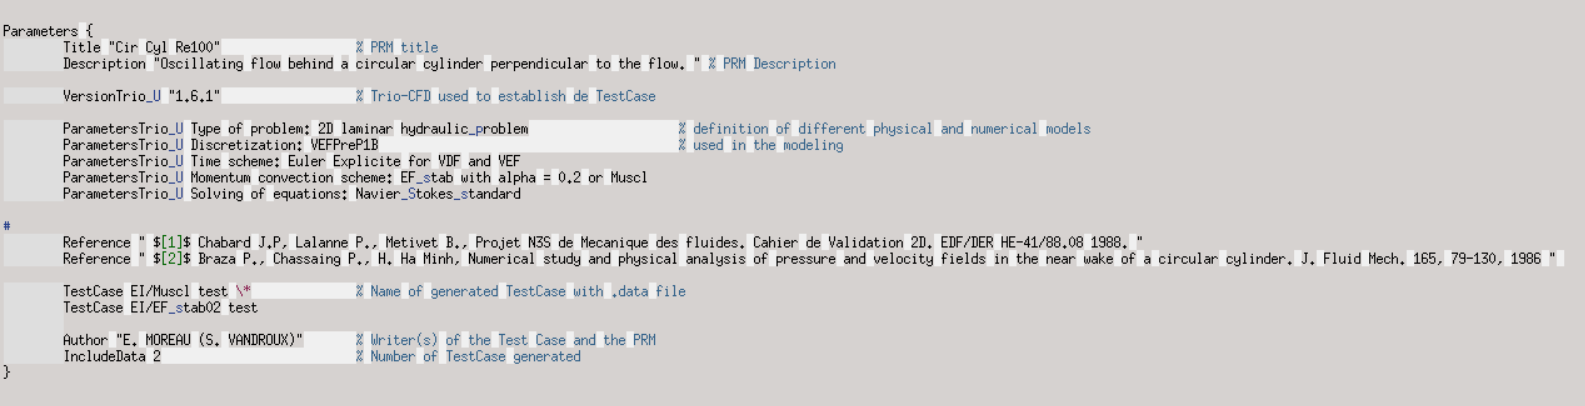
\includegraphics[width=16cm]{tools/parameters_PRM_1.png}\end{center}
\begin{center}\captionof{figure}{Original PRM syntax version - Parameters part}\end{center}

This part generates the first section of the PRM pdf entiteled \textit{1. Introduction} as follows:\newline
\setlength{\columnseprule}{0.5pt}
\begin{multicols}{2}
\begin{flushleft}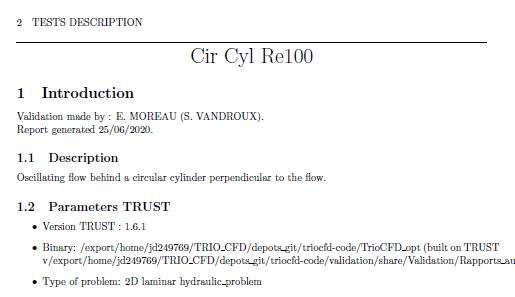
\includegraphics[width=8cm]{tools/parameters_PRM_1_pdf.png}\end{flushleft}
\columnbreak
\vspace{0.5cm}\begin{flushright}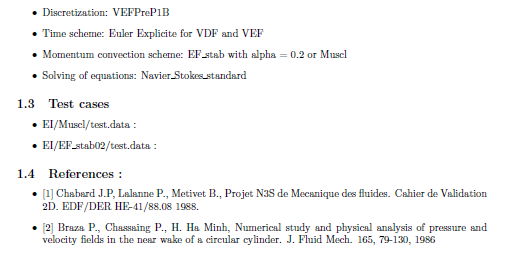
\includegraphics[width=8cm]{tools/parameters_PRM_2_pdf.png}\end{flushright}
\end{multicols}
\begin{center}\captionof{figure}{Original PRM syntax version - Generated introduction}\end{center}

After this first part, as many chapters as necessary can be added via the keword \verb"Chapter{ ... }" as follows:\newline
\begin{center}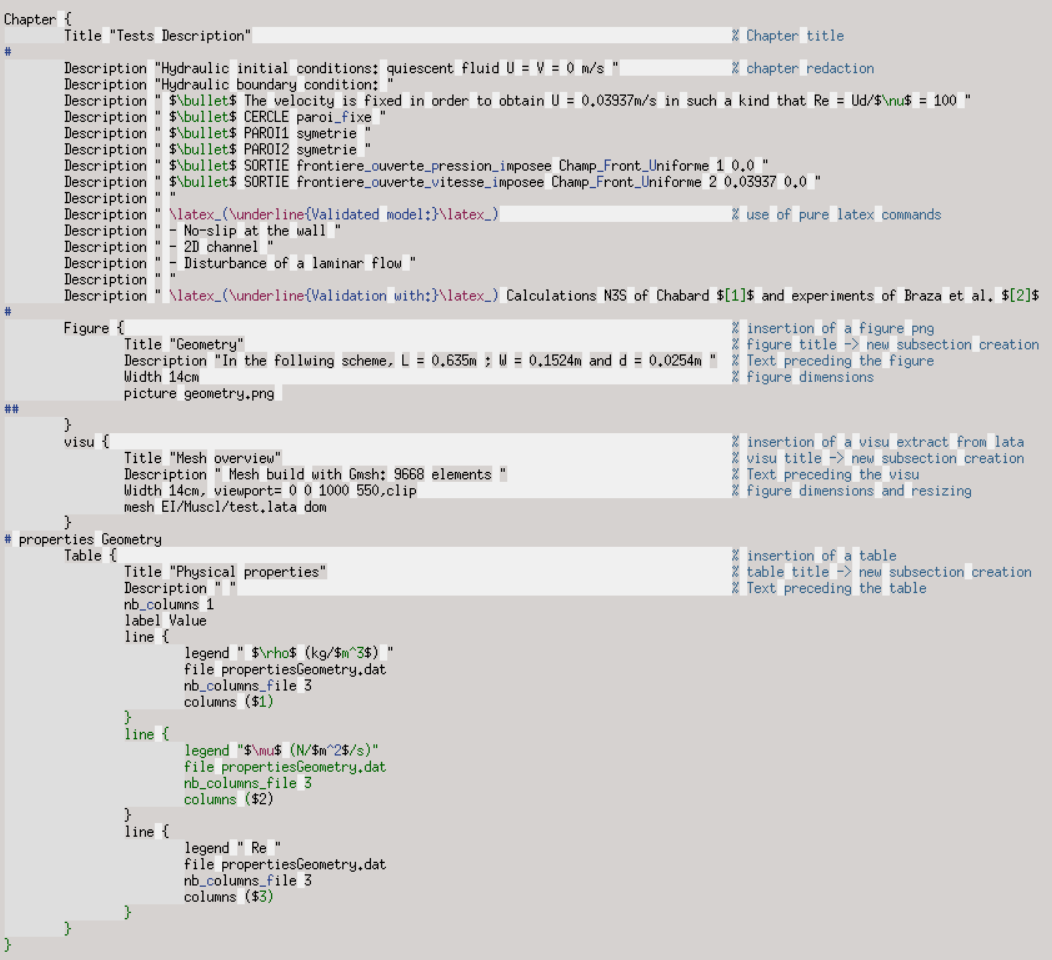
\includegraphics[width=12cm]{tools/chapter_PRM_1.png}\end{center}
\begin{center}\captionof{figure}{Original PRM syntax version - Chapter part}\end{center}

This part generates the second section of the PRM pdf entiteled \textit{2. Tests Description} as follows:\newline
\begin{center}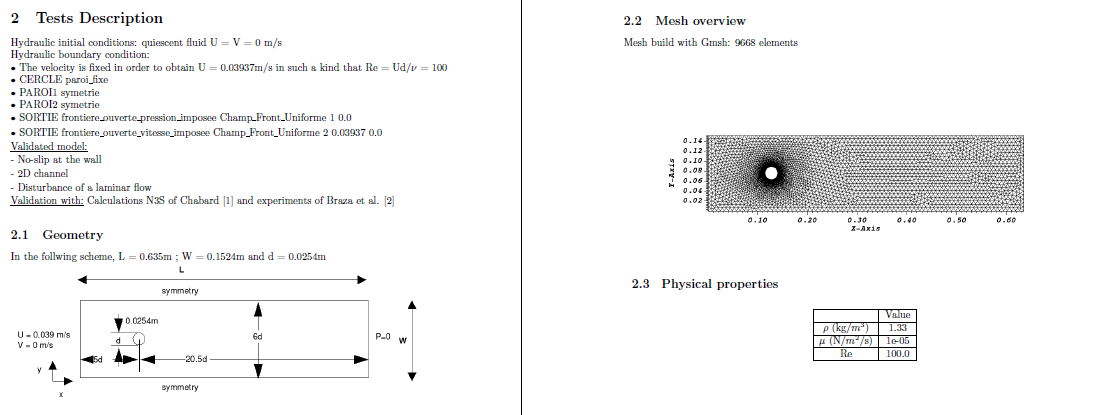
\includegraphics[width=15cm]{tools/chapter_PRM_1_pdf.png}\end{center}
\begin{center}\captionof{figure}{Original PRM syntax version - Generated chapter}\end{center}

You can find in Appendix A, the complete PRM as well as the pdf generated via the \verb "Run_fiche"  command with this unique model available in version v.1.8.1 of TRUST.\newline

%%%%%%%%%%%%%%%%%%%%%%%%%%%%%%%%%%%%%%%%%%%%%%%%%%%%%%%%%%%%%%%%%%%%%%%%%%%%%%%%%%%%%%%%
\section{\label{sec:New-PRM-syntax}New \textsf{PRM} syntax}
\lhead{\textit{New-PRM-syntax}}
\rhead{\textit{METHODOLOGY}}
For the constitution of this validation report, it was necessary to improve the relevance of the content as well as the formalism of these sheets in order to:\vspace*{0.2cm}\newline
\hspace*{0.5cm}$\Rightarrow$ have sheets with the object of validation and all the models used clearly expressed;\vspace*{0.15cm}\newline
\hspace*{0.5cm}$\Rightarrow$ have a harmony of structures between them.\vspace*{0.4cm}\newline
In this aim, improvements have been made to the general version of the \verb"Run_fiche" procedure (managed by the TRUST code) and a new tag has been created to activate the new formalism defined for Trio-CFD.\newline

\subsection*{General improvements}
Some modifications have been made in this new version for the generation of the latex from the PRM file without this affecting the way of writing the PRM.
Thus, the PRM always includes the first part entitled \textit{Parameters} as explained in chapter II.1, followed by as many chapters as desired by the writer via the \textit{Chapter} tag.\newline
The changes made concern two aspects:\vspace*{0.2cm}\newline
\hspace*{0.5cm}$\Rightarrow$ \textbf{Headers and footers:}\vspace*{0.15cm}\newline
Before, the left header of the pdf mentioned the numbers and titles of the last section and sub-section of the current page and the left footer, the name of the test case.\newline
Now, the left header contains the name of the test case and the left footer is empty. The right footer contains, as before, the page number. This reformatting allows better readability and was necessary for the concatenation of the latex into a single document.\vspace*{0.2cm}\newline
\hspace*{0.5cm}$\Rightarrow$ \textbf{Legend of figures and tables:}\vspace*{0.15cm}\newline
As seen in the previous chapter, adding a figure, a visu or a table automatically created a subsection with the name of the title of the figure (or visu or table) given in the PRM. Too many irrelevant subsections were created. The figures did not have a legend and
the title served as a caption.\newline
The python scripts have been modified so that the \textit{Title} fields of figures, visu and tables now correspond to the legend (fills in the Latex command \textit{captionof}) and their creation no longer generates a subsection.\newline

\subsection*{New formalism}
In addition to these general changes, a new formalism for validation sheets has been created. Its goalis to have an identical structure for all TrioCFD code validation sheets. This uniformity makes it possible to have a better readability of the validation sheets so that the users can quickly find which diagrams are to be used to model a particular phenomenon.
All validation sheets will therefore have the following structure:\medskip\newline
\setlength{\tabcolsep}{0.1cm}
\renewcommand{\arraystretch}{1.75}
\begin{tabular*}{16cm}{|m{5.75cm}|m{6.5cm}|m{3.25cm}|}
\hline
\textcolor{blue}{\textbf{Paragraph}} & \textcolor{blue}{\textbf{Description}} & \textcolor{blue}{\textbf{Keyword}} \\ \hline
\textbf{1. Purpose} & explains which models will be validated in the sheet and against which other results (numerical, analytical,...) the TrioCFD results will be validated& \textbf{purpose} or \textbf{objectif} \\ \hline
\textbf{2. Problem description} & & \textbf{pb\_description} \\
\hspace{0.2cm} 2.1 Geometry & describes the geometry of the physical domain defined to model the phenomenon & \textbf{geometry} or \textbf{geometrie} \\
\hspace{0.2cm} 2.2 Initials Conditions and Boundary Conditions & clarifies the initial conditions and the boundary conditions used in the modelization & \textbf{icbc} or \textbf{cicl} \\
\hspace{0.2cm} 2.3 Fluid Properties & gives the properties of the fluid considered& \textbf{fluidprop} or \textbf{propfluide} \\
\hspace{0.2cm} 2.4 Flow Physics & & \textbf{flowphy} or \textbf{phyecou} \\ \hline
\textbf{3. Case Setup} & & \textbf{casesetup} or \textbf{description\_cas} \\
\hspace{0.2cm} 3.1 Grid & describes the mesh(s) used for the calculations & \textbf{grid} or \textbf{maillage} \\
\hspace{0.2cm} 3.2 Model Options & & \textbf{model\_options} or \textbf{options\_modele} \\
\hspace{0.2cm} 3.3 Other Options (calculation) & & \textbf{other\_options} or \textbf{autres\_options} \\ \hline
\textbf{4. Results} & & \textbf{results} or \textbf{resultats} \\
\hspace{0.2cm} 4.1 Validation Specific Informations & recapitulates the main information of the file: version on which the sheet was established, digital models, CPU time, ... & \textbf{none} - automatically generated by the block \textit{Parameters} \\
\hspace{0.2cm} 4.2 Plot Data & & \textbf{none} - automatically generated if the block \textit{Results} is defined \\ \hline
\textbf{5. Conclusion} & & \textbf{conclusion}\\ \hline
\textbf{6. References} & lists the references cited in the sheet & \textbf{Reference} in the block \textit{Parameters} \\ \hline
\textbf{7. Data Files} & & \textbf{TestCase} in the block \textit{Parameters} if followed by \textbackslash\textasteriskcentered \\ \hline 
\end{tabular*}
\begin{center}\captionof{table}{New PRM syntax version - General structure}\end{center}

It can be activated by a specific keyword \textbf{newvalidTrio} to be defined at the top of the block \textit{Parameters} as follows:\newline
\begin{center}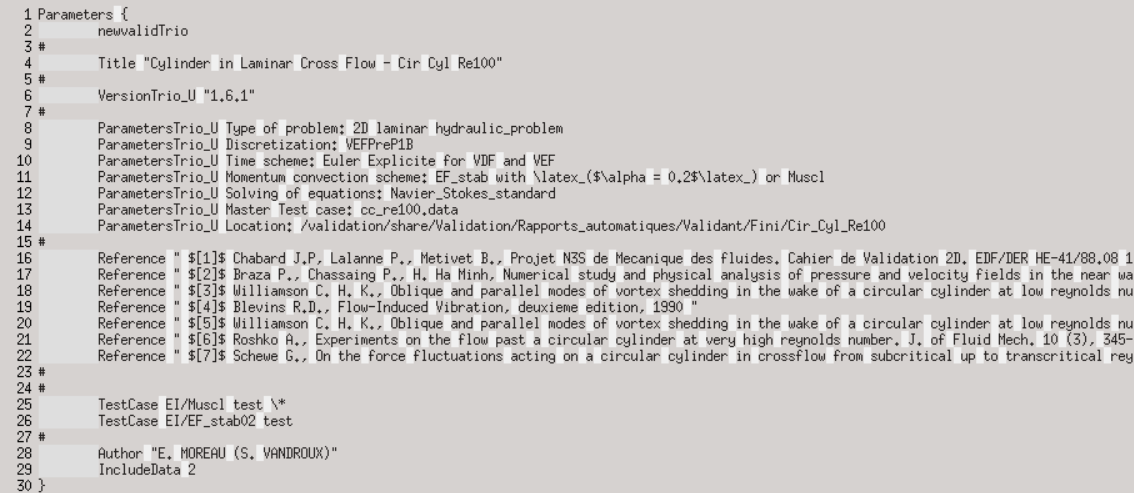
\includegraphics[width=16cm]{tools/parameters_PRM_1_newvalid.png}\end{center}
\begin{center}\captionof{figure}{New PRM syntax version - Parameters part}\end{center}

The first block is the block \textit{Parameters} which differs little from the previous version in terms of definition. It is constructed as follows :\smallskip\newline
$\Rightarrow$ keyword \textbf{newvalidTrio} : specific keyword which activates the new formalism \newline
$\Rightarrow$ keyword \textbf{Title} : defines the name of the validation sheet \newline
$\Rightarrow$ keyword \textbf{VersionTrio\_U} : gives the TrioCFD version from which the validation form was built. It is therefore not necessarily functional on earlier versions of the code \newline
$\Rightarrow$ keyword \textbf{ParametersTrio\_U} : \newline
$\Rightarrow$ keyword \textbf{Reference} : \newline
$\Rightarrow$ keyword \textbf{TestCase} : \newline
$\Rightarrow$ keyword \textbf{Author} : \newline
$\Rightarrow$ keyword \textbf{IncludeData} : \newline
The keyword \textbf{Description}, available in the inital formalism, is no longer taken into account.\smallskip\newline

In the inital formalism, \textit{Chapter} block was defined as many time as necessary with a title chosen by the writer of the validation sheet (see Chapter II.1). With this new formalism, predefined blocks can be used after the block \textit{Parameters}.\smallskip\newline
The second block (if the writer want to fill it up) is \textit{Problem description} block which can be activated by the keyword \textbf{pb\_description}.

%%%%%%%%%%%%%%%%%%%%%%%%%%%%%%%%%%%%%%%%%%%%%%%%%%%%%%%%%%%%%%%%%%%%%%%%%%%%%%%%%%%%%%%%
%%%%%%%%%%%%%%%%%%%%%%%%%%%%%%%%%%%%%%%%%%%%%%%%%%%%%%%%%%%%%%%%%%%%%%%%%%%%%%%%%%%%%%%%
\chapter{\label{chap:Validation-report-generation}\LaTeX~files and report generation}
